\documentclass[a4paper,12pt]{article}
% bitte diese Zeilen so lassen ------------------------
\usepackage[OT1]{fontenc}
\usepackage[utf8]{inputenc}
\usepackage{graphicx}
\usepackage{amsmath}
\usepackage{amssymb}
\usepackage{braket}

\usepackage{algorithm2e}
\parindent0em
\parskip1.5ex plus0.5ex minus0.5ex
\textwidth160mm
\textheight250mm
\renewcommand{\textfraction}{0}
\renewcommand{\bottomfraction}{1}
\renewcommand{\topfraction}{1}
\hoffset-2cm
\voffset-2cm
%\bibpunct{[}{]}{,}{n}{}{,}
% -----------------------
% hier eigene Definitionen

% -----------------------------------------------------
\begin{document}

% 1. Titelseite .......................................
\thispagestyle{empty}
\begin{minipage}{88mm}
\includegraphics{Logo_komplett_grau_links_400.pdf}
\end{minipage}\hfill
\begin{minipage}{70mm}
\begin{flushright}
{\sf
Fakultät für Physik\\
Friedrich-Hund-Platz 1\\
37077 Göttingen}
\end{flushright}
\end{minipage}
%\vspace{2mm}
\hrule
\vspace{-5mm}
\begin{flushright}
{\sf http://www.bachelor-fp-physik.uni-goettingen.de/}
\end{flushright}
%\hrule
\vspace{20mm}

\begin{center}
{\sffamily\bfseries\Huge Bachelor Fortgeschrittenenpraktikum}

% entsprechende Zeile auskommentieren
% {\sffamily\Large Schwerpunkt Astro- und Geophysik (M.phy.401)}
{\sffamily\Large Schwerpunkt Biophysik und Komplexe Systeme (B.phy.402)}
%{\sffamily\Large Schwerpunkt Festk"orper- und Materialphysik  (M.phy.403)}
%{\sffamily\Large Schwerpunkt Kern- und Teilchenphysik  (M.phy.404)}

% Hier das Versuchskuerzel in GRoßbuchstaben definieren
\newcommand{\vk}{B8.MDS}
% Hier den Versuchstitel definieren
\newcommand{\vt}{Frequenzanalyse von Vielteilchensystemen}
% Hier die Version (Jahreszahl+fortlfd. Nr+Sprache (D,E) definieren
\newcommand{\vv}{2012.09/A}
% Hier das Institut eintragen
\newcommand{\vi}{Max-Planck-Institut für biophysikalische Chemie}
% Hier den/die Verfasser eintragen
\newcommand{\va}{Timo Graen}

\vspace{\fill}

% auskommentieren für Bild:
% \includegraphics[width=140mm]{logo.png}
\includegraphics{oscillators.png}
\vspace{\fill}

{\sffamily\Large Versuchsanleitung zu \vk}

{\sffamily\bfseries\Huge
\vt\\}

\vspace{25mm}

\hrule
{\sffamily
\begin{tabular}{p{40mm}p{130mm}}
{\bfseries \vk} & \vi\\
Version \vv & Autor: \va\\
 & Assistent: \va \ (tgraen@gwdg.de)\\
 & Prüfer: Prof. Dr. Helmut Grubmüller
\end{tabular}

}

\end{center}
\newpage
% 2. Kurze Zusammenfassung .....................

\section*{Einleitung}
Proteine sind die Arbeitstiere der Natur und als solche hochspezialisierte Nanomaschinen. 
Sie sind von Menschen entworfenen Nanomaschinen noch weit überlegen, so existieren biomolekulare Motoren, Pumpen, selektive Kanäle, Signalgeber, etc.. 
Leider existieren in der Natur weder Bau- noch Gebrauchsanweisungen, welche uns Aufschluss über die molekularen Funktionsweisen liefern könnten. 
Die Erforschung der physikalischen Funktionsweise dieser Moleküle ist ein spannendes Gebiet der Biophysik und ähnelt stark dem Reverse Engineering 
in der Elektronik, basiert jedoch deutlich stärker auf der Statistischen- und Quantenphysik.

Ein großer Teil der Proteindynamik geschieht auf Zeit- und Längenskalen von fs-$\mu$s und 0.1-100 nm. Ein wünschenswerter Zugang zur 
Erforschung von Proteinfunktionen sind Molekulare Filme, also bewegte Bilder mit atomarer Auflösung. Leider existiert noch 
keine experimentelle Methode um die erforderlichen Zeit und Längenskalen aufzulösen.

Eine der zahlreichen experimentellen Methoden um trotzdem Informationen über die molekularen Prozesse der Proteinfunktion zu erlangen sind 
Infrarot Differenz Spektren. Hierbei wird versucht über die Unterschiede im Absorptionsverhalten von Proteinen im IR-Bereich
Informationen über Konformationsänderungen zu gewinnen. Dieser Frequenzbereich regt überwiegend Molekül Schwingungen an. Die resultierenden 
Differenzspektren enthalten die gewünschten Informationen sind jedoch schwierig zu interpretieren.

Ziel des Versuches ist es, zwei theoretische Methoden zur Berechnung von Protein Infrarot (Differenz-)Spektren kennenzulernen. Anhand von Wasser 
und zwei kleinen Proteinen wird die harmonische Normal Moden Analyse, sowie die Zeitreihen basierte Dipol-Autokorrelationsmethode eingeführt. Wir 
untersuchen das 'Gedächtnis' von Wasser und helfen einem befreundeten Chemiker ein Infrarot Absorption Experiment zu entwerfen.

\section{Frequenzanalyse} 
In diesem Versuch werden zwei Methoden zur Frequenz- oder Spektralanalyse vorgestellt. Ein schönes Beispiel \footnote{Beispiel inspiriert von Peter Hamms Buch: ISBN 978-1-107-00005-6}
für eine Frequenzanalyse ist das Spektrum eines teilweise gefüllten Weinglases. Eine Möglichkeit ein Spektrum zu erhalten ist mit dem Finger in
fester Umlaufzeit den Glasrand anzuregen. Wiederholt man dieses Vorgehen für viele Anregungsfrequenzen, so erhält man zusammen mit der Schallantwort
des Glases ein Resonanzfrequenzspektrum. Dieses ist jedoch nicht die einzige Möglichkeit. 

Eine weitere Möglichkeit ist das Glas anzustoßen und den entstehenden Ton Fourier zu zerlegen. Das Fourierspektrum des Glases ist, bis auf 
Messungenauigkeiten, identisch mit dem Spektrum durch Anregung mit dem Finger. Diese Methode entspricht der Dipol-Autokorrelationsmethode aus 
dem zweiten Versuchsteil. Bei dieser Methode werden die Schwingungsfreiheitsgrade des Proteins durch thermische Energie, also der thermischen 
Energie bei Raumtemperatur, angeregt. Die Konsequenz ist, dass sich das Protein zu bewegen beginnt. Einige dieser Bewegungen sind schnelle Schwingungen 
andere sind langsamere Konformationsänderungen. Diese Bewegungen können ebenfalls Fourier zerlegt werden, hierzu wird das Dipolmoment des gesamten Proteins 
aufgezeichnet und anschließend Fourier zerlegt. Die Wahl des Dipolmoments als Observable ist mehr oder weniger willkürlich, jedoch lässt sich 
das Dipolmoment Spektrum mit dem experimentell gemessen Spektrum vergleichen, siehe Kapitel \ref{dipolespec}. Das Protein in diesem Versuch 
wird durch klassische Punktteilchen und ein semi-empirisches Potential, das force field, beschrieben. Das resultierende Dipolmoment Spektrum misst also
auch die klassische Verteilung von thermischer Energie im Protein und berücksichtigt keine Nullpunktenergie hochfrequenten quantenmechanischer 
Schwingungen. Es handelt sich hier also auch um ein genähertes Spektrum.


Die Normal Moden Analyse (NMA) ist etwas schwieriger anhand des Weinglases zu erklären. In einer NMA nähern wir das Potential des Weinglases als Überlagerung
ungekoppelter harmonischer Oszillatoren mit Potential
\begin{equation}
 V(x_i)=\frac{1}{2} m_i \omega_i^2 x_i^2.
\end{equation}
Hierbei ist $\omega_i$ die Kreisfrequenz des harmonischen Oszillators $i$ und $x_i$ die Auslenkung aus der Ruhelage. Die Masse $m_i$ ist schwierig zu definieren, 
da es sich ja nicht um einzelne schwingende Massenpunkte handelt. Im Kapitel \ref{nmasection} wird gezeigt, wie die Massen $m_i$ mit in die kollektiven Koordinaten
$x_i$ integriert werden können.
Nehmen wir nun an, dass das Weinglas in $x,y,z$ Richtung schwingen kann, dann würde unser harmonisches Weinglas aus drei Oszillatoren bestehen. Das entsprechende 
Spektrum hätte drei Frequenzen. In einem Protein würden wir jedem Atom diese drei Freiheitsgrade zuordnen, sodass für $N$ Atome $3N$ Oszillatoren benötigt werden.
Da in der Regel kein externes Potential anliegt, kann es keine gleichzeitige periodische Bewegung (Translation, Rotation) aller Atome in eine Richtung geben.
Aus diesem Grund betrachtet man meist $3N-6$ Freiheitsgrade, da sechs Frequenzen Null sein müssen. 
Die Kreisfrequenzen $\omega_i=\sqrt{\frac{k_i}{m_i}}$ können wir aus den Kraftkonstanten $k_i$ 
zu diesen Schwingungen bestimmen, indem wir an dem Glas in den drei Raumrichtungen $\Delta x$ ziehen und die Kraft 
\begin{equation}
 F_i=-k_i \Delta x
\end{equation}
messen. 

Es ist schnell ersichtlich, dass für die Normal Moden Analyse eine sehr empfindliche Näherung gemacht wird. Diese ist exakt für harmonische Systeme
wie zum Beispiel die unendliche Kette harmonischer Oszillatoren, oder die geschlossene Kette. Proteine sind leider meistens nicht harmonisch, weshalb
das Spektrum der Normal Moden Analyse sehr große Abweichungen von experimentellen Messungen haben kann.



\section{Theorie Normal Moden Analyse}\label{nmasection}
Die Normal Moden Analyse (NMA) berechnet die Eigenfrequenzen eines Vielteilchensystems in harmonischer Näherung. Das bedeutet, dass sämtliche 
Ergebnisse der NMA ausschließlich für vollständig harmonische Systeme exakt sind. Das exakte Potential $V(r_i)$ für $N$ Teilchen muss zerlegbar 
sein in
\begin{equation}
 V(x_i)=\sum_i^N c_i x_i^2
\end{equation}
mit $c_i=\frac{1}{2}m_i \omega_i^2$. $m_i$ sind die Atommassen und $\omega_i$ die Frequenzen zur Koordinate $x_i$. Für alle anderen Potentiale ist 
die NMA eine mehr oder weniger gute Näherung. Die Qualität der Ergebnisse wird besonders in der chemischen Literatur häufig überschätzt.

Alternativ kann die NMA physikalisch auch als harmonisches Glied in der Taylorreihe eines beliebigen Potentials 
\begin{equation}
 V=V_0+\sum_i^N \left( \frac{\partial V}{\partial x_i} \right) x_i + \frac{1}{2} \sum_i^N \sum_j^N \left( \frac{\partial^2 V}{\partial x_i \partial x_j} \right) + \ldots
\end{equation}
betrachtet werden. Es muss noch eine geeignete Konfiguration gewählt werden, um welche entwickelt wird. Hierfür bietet sich die Konfiguration beim absoluten Temperatur Nullpunkt
bei 0 K an, unter der Annahme, dass die Teilchen klassisch sind. Die Nullpunktenergie definieren wir als Referenzenergie $V_0=0$ und die erste Ableitung ist per Definition 
des Energieminimums $\frac{\partial V}{\partial x_i}=0$. Damit verbleibt für kleine Auslenkungen von der Nullpunkt Struktur
\begin{equation}
 V\approx\frac{1}{2} \sum_i^N \sum_j^N \left( \frac{\partial^2 V}{\partial x_i \partial x_j} \right).
\end{equation}
Ein einfacher Algorithmus, um das nächstliegende Energieextremum zu finden ist zum Beispiel Steepest Descent:

\begin{algorithm}[H]
 \SetAlgoLined
 \KwData{Minimalistischer Energie Minimierer: Steep Algorithm}
 $x_{old} = 0$\;
 $x_{new} = x_{init}$\;
 $F_{scale} = 0.001$;  force scaling factor\;
 $precision = 0.00001$; stop, if the displacement in structure is smaller than this\;	
 \While{$ |x_{new} - x_{old}| > precision$:}{
     $x_{old} = x_{new}$\;
     $x_{new} = x_{old} - F_{scale} \cdot Calc\_Forces(x_{old})$\;
 }
 \caption{Minimiert die Ableitung des Potentials (Kraft $F=-\nabla V$) als Vorbereitung für NMA. }
\end{algorithm}
\begin{figure}[ht!]
 \centering
 \includegraphics[scale=0.5,keepaspectratio=true]{./nma.pdf}
 % nma.pdf: 563x237 pixel, 72dpi, 19.86x8.36 cm, bb=0 0 563 237
 \caption{Gekoppelter Harmonischer Oszillator, Massen $m_i$, Kraft Konstanten $k_i$ und Positionen $x_i$}
 \label{fig:hos}
\end{figure}
Sobald die Struktur vorliegt verhält sich der Rest der Analyse analog zum gekoppelten harmonischen Oszillator.
Wir benutzen einige Eigenschaften des Harmonischen Oszillators $V=\frac{1}{2}kx^2$:
\begin{equation}
 F=-\frac{dV}{dx}=-kx=ma=m\frac{d^2x}{dt^2}
\end{equation}
und damit ergibt sich durch Einsetzen der Lösung
\begin{equation}
 x(t)=Asin(\omega t),
\end{equation}
sowie
\begin{equation}
 k=-\frac{d^2V}{dx^2}
\end{equation}
die Oszillator Gleichung
\begin{equation}
 m \omega^2 x = k x.
\end{equation}

Für das gekoppelte System aus Figure \ref{fig:hos} folgt damit das Gleichungssystem

\begin{eqnarray}
 \omega^2 m_1 x_1 &=& k_{x_1,x_1} x_1 +k_{x_1,x_2} x_2\\
 \omega^2 m_2 x_2 &=& k_{x_2,x_1} x_1 +k_{x_2,x_2} x_2,
\end{eqnarray}
oder equivalent 
\begin{eqnarray}
 \omega^2 \sqrt{m_1} x_1 &=& \frac{ k_{x_1,x_1} }{ \sqrt{m_1} } x_1 +\frac{ k_{x_1,x_2} }{ \sqrt{m_1} } x_2\\
 \omega^2 \sqrt{m_2} x_2 &=& \frac{ k_{x_2,x_1} }{ \sqrt{m_2} } x_1 +\frac{ k_{x_2,x_2} }{ \sqrt{m_2} } x_2.
\end{eqnarray}

Welches mittels der Abkürzungen $\overline{x}_i=\sqrt{m_i}x_i$ und $\overline{k}_{x_i,x_j}=\frac{{k}_{x_i,x_j}}{\sqrt{m_i}\sqrt{m_j}}$
zu
\begin{eqnarray}
 \omega^2 \overline{x}_1 &=& \overline{k}_{x_1,x_1} \overline{x}_1 +\overline{k}_{x_1,x_2} \overline{x}_2\\
 \omega^2 \overline{x}_2 &=& \overline{k}_{x_2,x_1} \overline{x}_1 +\overline{k}_{x_2,x_2} \overline{x}_2,
\end{eqnarray}
oder
\begin{equation}
 \omega^2 
 \hat{\overline{x}} = 
 \begin{pmatrix}
  \overline{k}_{x_1,x_1} &\overline{k}_{x_1,x_2}\\
  \overline{k}_{x_2,x_1} &\overline{k}_{x_2,x_2}
 \end{pmatrix}
 \hat{\overline{x}}
\end{equation}
vereinfacht werden kann. Wichtig ist, dass das Ziel dieser Umformung das Auffinden von koherenten Bewegungen, also Bewegungen welche in
Phase mit der gleichen Frequenz schwingen, mehrerer Atome ist. Daher gibt es nur $\omega$ und nicht $\omega_i$ in den oben stehenden
Gleichungen. Die Eigenwerte dieser Gleichung $\omega_i^2$ sind jedoch das Quadrat der gesuchten $3N-6$ Harmonischen 
Eigenfrequenzen $\omega_i$ des Systems. Zusätzlich erhält man in der NMA einen vollständigen Satz an Eigenvektoren $\Omega_i$, 
welche jedoch immer noch in Massen gewichteten Koordinaten vorliegen und die Dimension [Masse$^{1/2}$ Länge] haben.
\section{Infrarot Absorption im Experiment}
\begin{figure}[ht!]
 \centering
 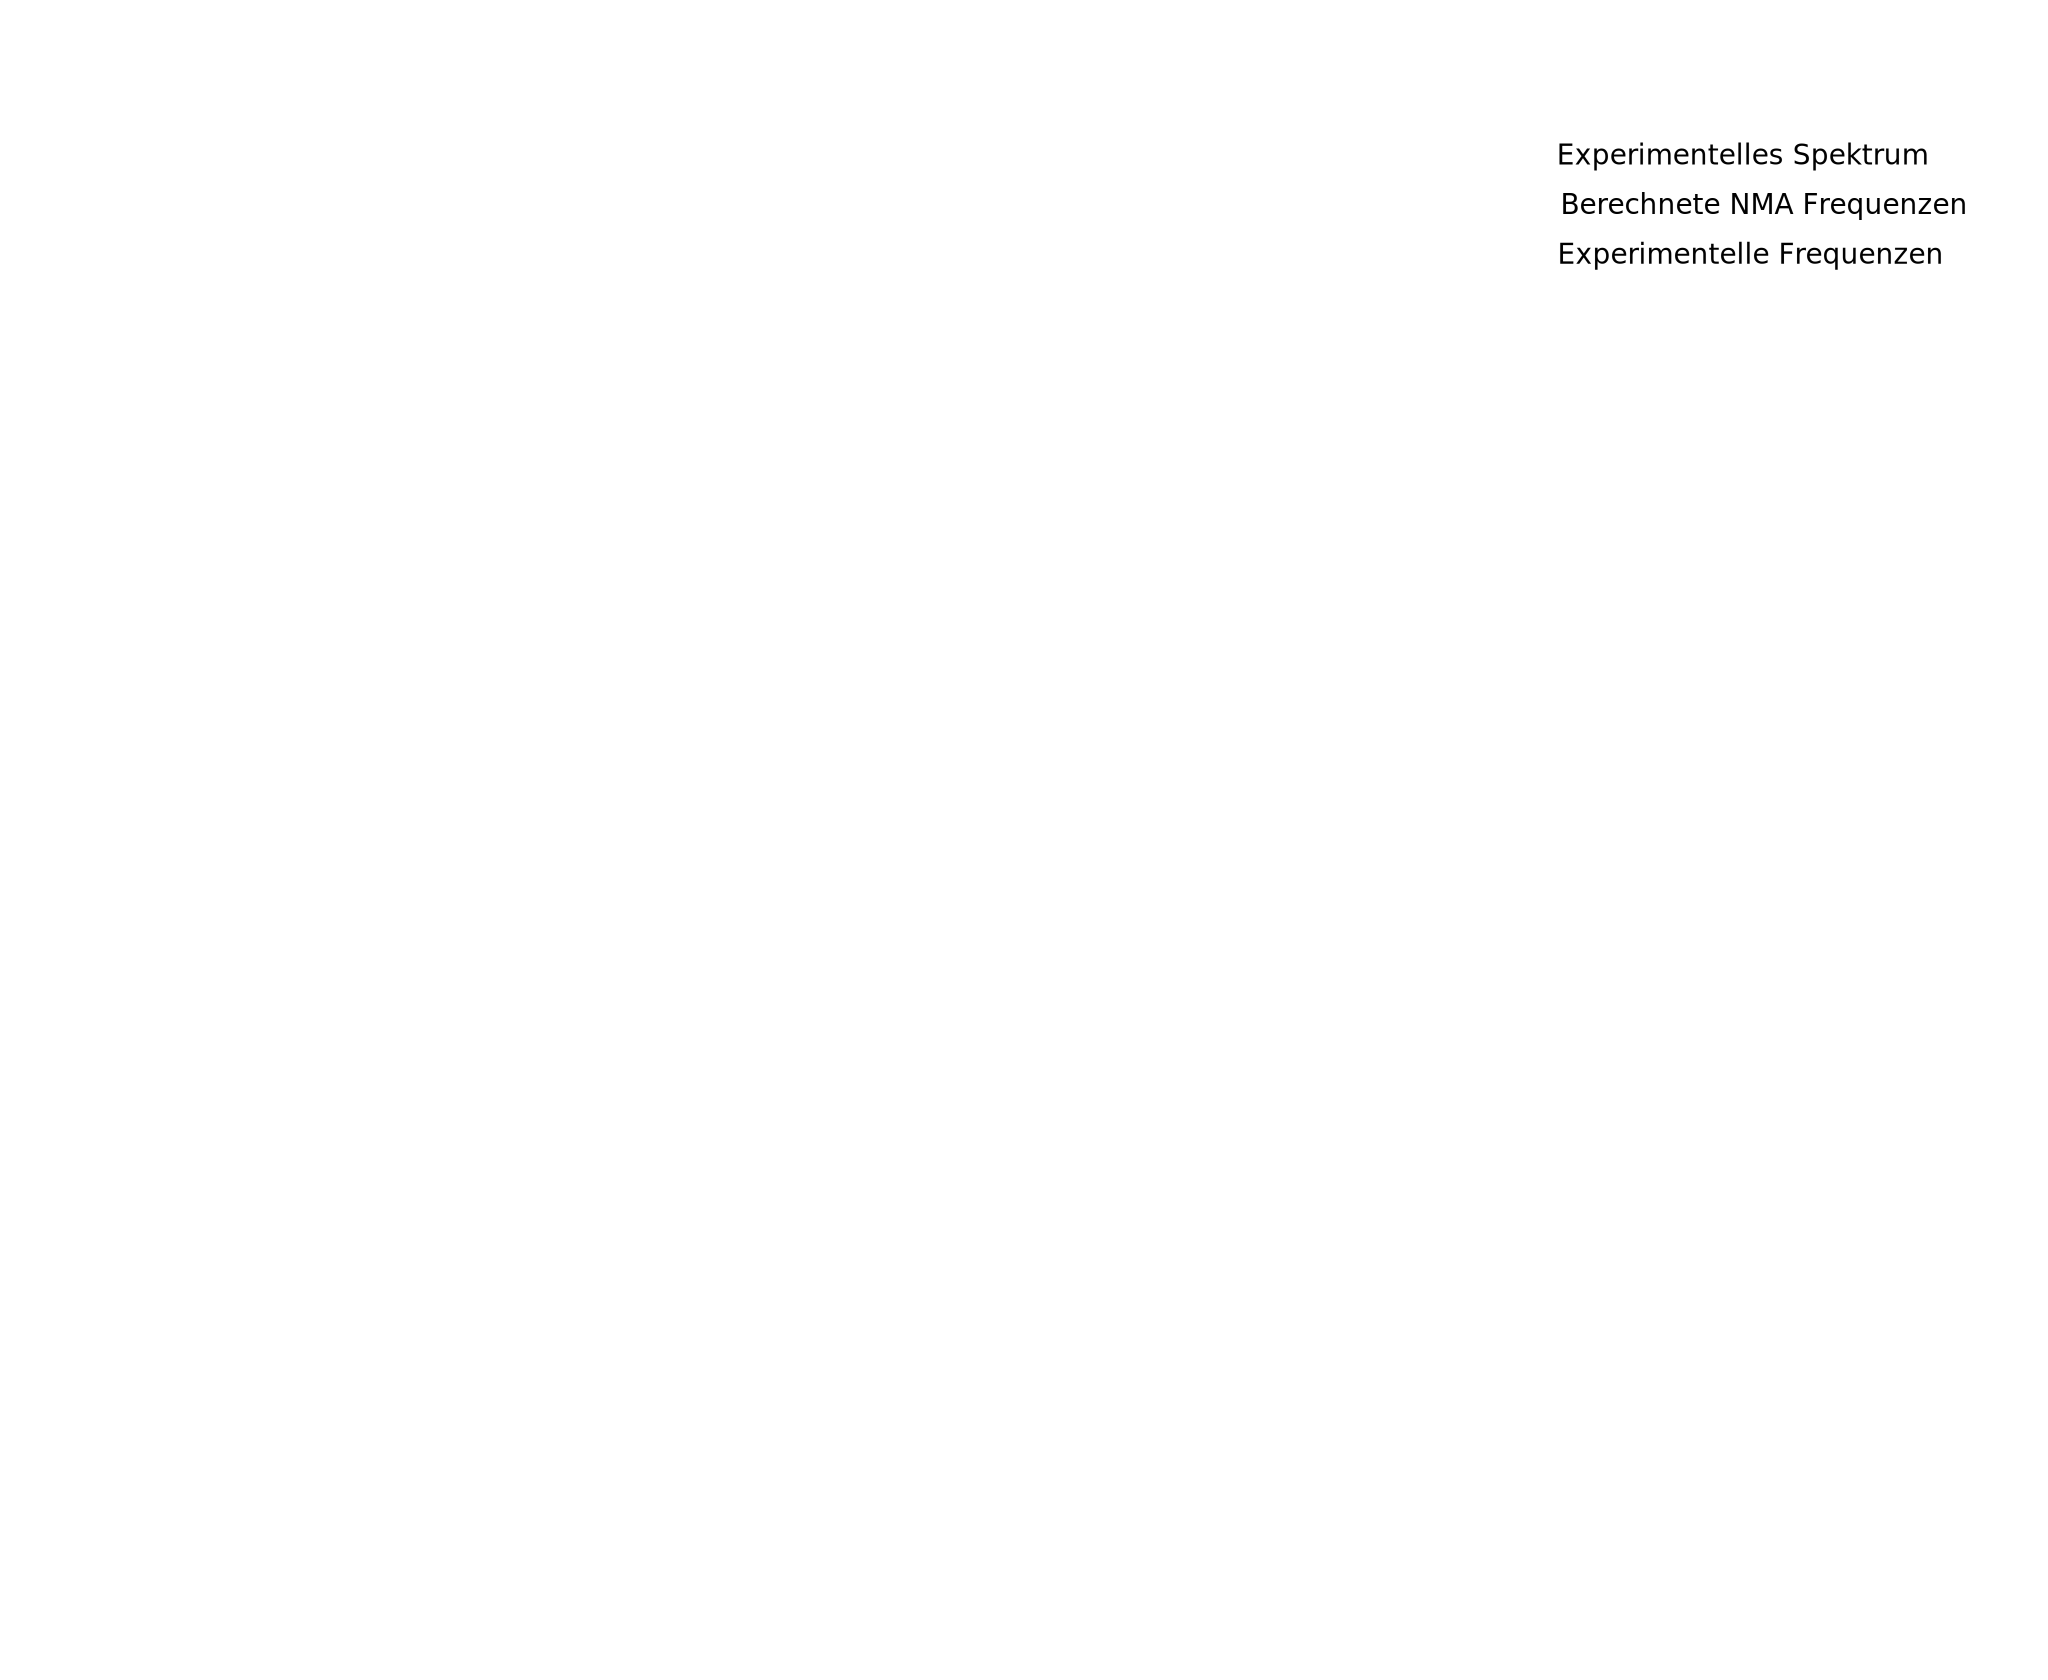
\includegraphics[scale=0.2,keepaspectratio=true]{./spektrum_exp_nma.png}
 % spektrum_exp_nma.png: 2109x1731 pixel, 72dpi, 74.40x61.07 cm, bb=0 0 2109 1731
 \caption{Illustration eines Infrarot Spektrums mit eingezeichneten NMA Frequenzen. Es ist deutlich zu sehen, dass die Absorptionsintensität nicht für alle Frequenzen gleich ist und die harmonischen 
  NMA Frequenzen nicht exakt mit den experimentellen Frequenzen übereinstimmen.
  Die Einheit $cm^{-1}$ wird als Wellenzahl oder wavenumber bezeichnet und ist eine übliche Spektroskopie Einheit und wird aus Frequenz $f$ und Vakuum Lichtgeschwindigkeit $c$ durch $f/c$ berechnet. 
  }
 \label{fig:nma_exp_comp}
\end{figure}
Nach Berechnung der Eigenfrequenzen $\omega_i$ und Eigenvektoren $\Omega_i$ in Abschnitt \ref{nmasection} bleibt noch der Bezug zum 
Experiment. In Infrarot Absorptions Messungen wird bestimmt, welche und wie stark Frequenzen von einem Protein absorbiert werden. Aus
der Kenntnis des Eingangssignals und der gemessenen Transmission kann dann das gemessene Absorptionsspektrum bestimmt werden. 

Die theoretisch bestimmten Schwingungsfrequenzen $\omega_i$ aus Abschnitt \ref{nmasection} können schon mit dem Experiment verglichen 
werden, jedoch kann noch keine Aussage über die Absorptionsintensität getroffen werden. Abbildung \ref{fig:nma_exp_comp} ist eine Illustration,
welche die Unterschiede in der Absorptionsintensität veranschaulicht.

Die Berechnung der Absorptionsintensität ist ein wenig komplizierter als die Berechnung der Frequenzen. In erster Näherung wechselwirkt das 
elektrische Feld $\vec{E}(x,t)=\vec{E}_0(x)e^{-i\omega t}$ eines IR-Photons mit dem Dipolmoment $\vec{\mu}$ des Moleküls. Diese Wechselwirkung
wird als Störung 
\begin{equation}
\hat{H}'= \vec{\mu}\cdot \vec{E}(x,t)
\end{equation}
 des Molekül Hamilton Operators $\hat{H}_0$ betrachtet. So ergibt sich für den gesamt Hamilton Operator 
\begin{equation}
 \hat{H}=\hat{H_0}+\hat{H}'
\end{equation}

Dieser Gesamthamiltonian kann nun in die Zeitabhängige Schrödingergleichung 

\begin{equation}\label{schroedinger}
 \hat{H}\psi(x,t)=-\frac{\hbar}{i} \frac{\partial \psi(x,t)}{\partial t}
\end{equation}

eingesetzt werden und ergibt

\begin{equation}\label{schroedingerpert}
 (\hat{H}+\hat{H}')\psi'(x,t)=-\frac{\hbar}{i}\frac{\partial}{\partial t}\psi'(x,t).
\end{equation}


Die resultierende gestörte Wellenfunktion $\psi'(x,t)$ kann anschließend in der Basis der Eigenfunktionen $\psi_n(x,t)=\psi_n(x) e^{-iE_nt/\hbar}$ des ungestörten Hamilton Operators $\hat{H}$ ausgedrückt werden als
\begin{equation}\label{wfexpansion}
 \psi'(x,t)=\sum_n a_n(t) \psi_n(x) e^{-iE_nt/\hbar}.
\end{equation}
Die Entwicklungskoeffizienten $a_n(t)$ enthalten die gesuchte Information über die Wahrscheinlichkeit $p_m(t)=|a_m(t)|^2$ das ursprüngliche System $\psi_s(x)$ in dem finalen Zustand $\psi_m(x)$ 
nach Zeit $t$ zu finden. Dieser finale Zustand kann z.B. das System nach Absorption des Photons sein. Das Ziel ist es also im Folgenden Teil eine sog. Mastergleichung der Form
\begin{equation}
 \dot{a}_i=C a_i
\end{equation}
für die Koeffizienten herzuleiten. Als erstes setzen wir Gleichung \ref{wfexpansion} in Gleichung \ref{schroedingerpert} ein und erhalten
\begin{eqnarray}\label{perturbedfull}
  (\hat{H}+\hat{H}')\sum_n a_n(t) \psi_n(x) e^{-iE_nt/\hbar}&=&-\frac{\hbar}{i}\frac{\partial}{\partial t}\sum_n a_n(t) \psi_n(x) e^{-iE_nt/\hbar} \nonumber\\
              &=&-\frac{\hbar}{i}\sum_n \dot{a}_n(t) \psi_n(x) e^{-iE_nt/\hbar} \nonumber \\
              & &-\frac{\hbar}{i}\sum_n a_n(t) \frac{\partial}{\partial t} \psi_n(x) e^{-iE_nt/\hbar}.
\end{eqnarray}
Wir benutzen nun die Beziehung
\begin{eqnarray}\label{perturbedfull2}
  \sum_n a_n(t) \hat{H} \psi_n(x) e^{-iE_nt/\hbar} & =&-\sum_n a_n(t) \frac{\hbar}{i} \frac{\partial}{\partial t} \psi_n(x) e^{-iE_nt/\hbar}
\end{eqnarray}
und wenden sie auf den letzten Term in Gleichung \ref{perturbedfull} an. Wir erhalten nun einen vereinfachten Ausdruck für die Zeitableitung der Entwicklungskoeffizienten $a_n$,
\begin{eqnarray}
  \sum_n a_n(t)  \hat{H}'\psi_n(x) e^{-iE_nt/\hbar}&=&-\frac{\hbar}{i}\sum_n \dot{a}_n(t) \psi_n(x) e^{-iE_nt/\hbar}. 
\end{eqnarray}
Der Ausdruck lässt sich noch weiter vereinfachen, indem von links mit $\psi_m(x,t)$ multipliziert wird. Außerdem führen wir die Abkürzung
\begin{equation}
 E_{m,n} = (E_m-E_n)~=~\hbar\omega_{m,n}\nonumber\\ 
\end{equation}
ein und wechseln zur $\braket{bra | ket}$ Schreibweise, wodurch wir folgenden Ausdruck erhalten:
\begin{eqnarray}
  \sum_n a_n(t) \bra{\psi_m}\hat{H}'\ket{\psi_n} e^{i\omega_{m,n}t}&=& -\frac{\hbar}{i}\sum_n \dot{a}_n(t)\braket{\psi_m|\psi_n}  e^{i\omega_{m,n}t} \nonumber\\
  \sum_n a_n(t) \hat{H}'_{m,n} e^{i\omega_{m,n}t}&=&-\frac{\hbar}{i} \dot{a}_m(t).\label{hmncomplex}
\end{eqnarray}
Wir haben hier die Orthogonalitätsrelation $\braket{\psi_m |\psi_n}=\delta_{mn}$ benutzt und die Abkürzung für die Matrix Elemente 
$\hat{H}'_{m,n}=\bra{\psi_m}\hat{H}'\ket{\psi_n}$ eingeführt. 

Gleichung \ref{hmncomplex} ist lineares Gleichungssystem, welches die zeitliche Entwicklung der Koeffizienten $a_n$ beschreibt. Aus dieser Gleichung lassen sich die 
Absorptionswahrscheinlichkeiten $p_i$ bestimmen. Als erstes wird angenommen, dass die Störung $\hat{H}'$ klein und von kurzer Dauer ist. Dieses hat zur Folge,
das die Entwicklungskoeffizienten $a_i(t)$ durch ihren Wert bei $t=0$ genähert werden können, also $a_i(t)\approx a_i(t=0)$. Das System befindet sich zum Zeitpunkt
$t=0$ im Zustand $\psi(x,t=0)=\psi_s(x)$. Dieser Zustand soll Eigenzustand sein und wird beschrieben durch einen Koeffizientenvektor mit $a_i=0$ bis auf ein spezielles $a_s=1$. 
Daraus ergibt sich eine stark vereinfachte Version von Gleichung \ref{hmncomplex}, 
\begin{eqnarray}\label{hmncomplex2}
 \dot{a}_m(t)&=&-\frac{i}{\hbar} \hat{H}'_{m,s} e^{i\omega_{m,s}t} .
\end{eqnarray}
Für eine zeitabhängige Störung $\hat{H}'(t)=\hat{H}'e^{-i\omega t}$ mit Frequenz $\omega$ ändert sich Gleichung \ref{hmncomplex2} leicht zu
\begin{equation}\label{hmncomplex3}
 \dot{a}_m(t) = -\frac{i}{\hbar} \hat{H}'_{m,s} e^{i(\omega_{m,s}-\omega)t} .
\end{equation}
Wir können nun Gleichung \ref{hmncomplex3} auf dem Intervall $t'=[0..t]$ integrieren mit der Annahme, dass der finale Zustand $\ket{m}$ zur Zeit $t=0$ unbesetzt ist, also $a_m(t=0)=0$. 
Hieraus erhalten wir die Koeffizientengleichung
\begin{equation}\label{amsolution}
 a_m(t) = \frac{1}{\hbar} \hat{H}_{m,s}' \frac{1-e^{i(\omega_{m,s}-\omega)t}}{(\omega_{m,s}-\omega)}.
\end{equation}
Aus der Koeffizientengleichung \ref{amsolution} kann nun wie oben beschrieben, die Übergangswahrscheinlichkeit 
\begin{equation}\label{mastereq1}
 p_{m,s}(t)=|a_m(t)|^2 = \frac{2}{\hbar^2}|\hat{H}_{m,s}'|^2 \frac{1-cos((\omega_{m,s}-\omega) t)}{(\omega_{m,s}-\omega)^2}
\end{equation}
von Zustand $\ket{s}$ in den Zustand $\ket{m}$ mittels Lichtabsorption. 
In unserem Fall ist die Störung das elektrische Feld eines Photons $\vec{E}(x,t)=\vec{E}_0(x)e^{-i\omega t}$ welches mit dem Dipolmoment $\mu$ des Systems wechselwirkt,
\begin{equation}\label{perturbationE}
\hat{H}'=\vec{\mu}\cdot \vec{E}(x,t) 
\end{equation}
Die Wechselwirkung ist maximal, wenn Feld und Dipolmoment parallele Ausrichtung haben und Null für senkrechte Ausrichtungen. 

Setzten wir nun den Wechselwirkung \ref{perturbationE} in die Gleichung für die Übergangswahrscheinlichkeit \ref{mastereq1} ein, so erhalten wir die gesuchte Absorptionswahrscheinlichkeit
\begin{equation}\label{mastereq2}
 p_{m,s}(t)= \frac{2}{\hbar^2}|\bra{\psi_m} \vec{\mu} \ket{\psi_s} |^2 |\vec{E_0}|^2 cos^2(\theta_{\mu,E_0}) \frac{1-cos((\omega_{m,s}-\omega) t)}{(\omega_{m,s}-\omega)^2}.
\end{equation}
Diese Gleichung kann nun benutzt werden, um aus unsere NMA mit dem Experiment zu vergleichen.
Gleichung \ref{mastereq2} verknüpft die Übergangswahrscheinlichkeit $p_{m,s}$, oder auch Intensität $I_{m,s}$, mit dem Dipolmoment Operator $\vec{\mu}=\sum_i e_i \vec{x}_i$. $e_i$ 
ist die effektive Ladung von Atom i und $\vec{x}_i$ ist der Vektor von Atom $i$ in Bezug auf den Schwerpunkt des Systems. 
Wir sehen nun, dass die Intensität $I_{m,s}$ für den Übergang von Zustand $\ket{s}$ nach Zustand $\ket{m}$ 
\begin{equation}\label{intensityeq1}
 I_{m,s} \varpropto \left( [\hat{\mu}_x]^2_{m,s} + [\hat{\mu}_y]^2_{m,s} + [\hat{\mu}_z]^2_{m,s} \right),
\end{equation}
wobei
\begin{equation}\label{dipl1}
[\hat{\mu}_j]_{m,s}=\bra{\psi_m}\hat{\mu}_j \ket{\psi_s}. 
\end{equation}

Die Übergangsintensitäten können in harmonischer Näherung durch Taylor Entwicklung des Dipolmoment Operators entlang der NMA Eigenvektoren $\Omega_i$ berechnet werden
\begin{equation}\label{mutaylor}
 \vec{\mu} \approx  \vec{\mu}_0 + \sum_{i=1}^{3N-6} \left(\frac{\partial \vec{\mu}}{\partial \Omega_i}\right)_{\mu_0} \Omega_i.
\end{equation}
Für die Elemente $[\hat{\mu}_j]_{m,s}$ gilt:
\begin{eqnarray}\label{maximu}
  [\hat{\mu}_j]_{m,s}&=&\bra{\psi_m}\hat{\mu}_j \ket{\psi_s} \nonumber \\
                     &\approx&\bra{\psi_m} \mu_0 + \sum_{i=1}^{3N-6} \left(\frac{\partial \mu}{\partial \Omega_i}\right)_{\mu_0} \Omega_i \ket{\psi_s} \nonumber\\
                     &=&\mu_0 \underbrace{\braket{\psi_m|\psi_s}}_{=0} + \sum_{i=1}^{3N-6} \bra{\psi_m}  \left(\frac{\partial \mu}{\partial \Omega_i}\right)_{\mu_0} \Omega_i \ket{\psi_s} \nonumber\\
                     &=&\sum_{i=1}^{3N-6} \bra{\psi_m}  \left(\frac{\partial \mu}{\partial \Omega_i}\right)_{\mu_0} \Omega_i \ket{\psi_s}.
\end{eqnarray}

Diese letzte Gleichung kann nun in Gleichung \ref{mastereq2} eingesetzt werden, um die wichtige Verbindung zwischen Frequenzen $\omega_i$, Übergangsintensitäten $I_{m,s}$, und den NMA
Eigenvektoren $\Omega_i$ herzustellen, welche den Vergleich mit dem Experiment ermöglichen.
Die Änderung des Dipolmoments des Moleküls $\left(\frac{\partial \mu}{\partial \Omega_i}\right)_{\mu_0}$ in Richtung des Vektors $\Omega_i$ ist also (in harmonischer Näherung!) 
entscheidend dafür, wie stark eine bestimmte Schwingungsmode mit Frequenz $\omega_i$ Licht absorbiert.

\section{Theorie Dipole Moment Spektrum}\label{dipolespec}
Eine alternative Methode zur Berechnung eines IR-Absorptionsspektrums ist die Zeitreihenanalyse des Dipolmoments $\hat{\mu}(t)$ des Moleküls. Hierfür wird eine Molekulardynamik Simulation
des Systems bei einer Temperatur $T$ durchgeführt, z.B. $T=300K$. Während der Simulation wird der Dipolmoment Vektor $\hat{\mu}(t)$ aufgezeichnet. Im Nachfolgenden Teil berechnen wir die 
Absorptionsintensitäten, indem wir $\left(\frac{\partial \mu}{\partial \Omega_i}\right)_{\mu_0}$ aus der Zeitreihenanalyse des Dipolmoments der Simulationsbox berechnen. Anstelle der
Zeitreihe benutzen wir die Autokorrelationsfunktion der Zeitreihe, da diese nicht mehr explizit von der Simulationszeit $t$ abhängt. Durch die Verwendung der Autokorrelationsfunktion 
geht die relevante spektrale Information nicht verloren, jedoch reduzieren wir das Rauschen der Daten. Wir benutzten das Wiener-Khinchin Theorem, um aus der Zeitreihe 

  \begin{equation}
   \mu(t) = \left\{ 
         \begin{matrix}
          \mu(t) &  |t| < T\\
               0 &  |t| > T
         \end{matrix} 
         \right .
  \end{equation}
ein Spektrum $S(\omega)$ erzeugt. Hierfür benötigt man die Definition der Fouriertransformation des Signals $F(\omega)$ und ihr inverses 
  \begin{eqnarray}
   F(\omega)&=&             \int_{-\infty}^{\infty} \mu(t) e^{-i\omega t} dt\\
   \mu(t)   &=& (2\pi)^{-1} \int_{-\infty}^{\infty} F(\omega) e^{i\omega t} d\omega.
  \end{eqnarray}
Als nächstes nutzt man die Definition der Autokorrelationsfunktion 
  \begin{equation}
   R(\tau)=E[\mu^*(t) \mu(t+\tau)],
  \end{equation}
wobei $E[]$ das Ensemblemittel ist. Wir nehmen im weiteren Verlauf Ergodizität an, wobei dieses auch dem Zeitmittel entspricht. 
Mit Hilfe der spektralen Leistungsdichte (Power Spectral Density) 
  \begin{equation}\label{preKWT}
   S(\omega) = \lim_{T\rightarrow\infty} \frac{1}{2T} E[|F_T(\omega)|^2]
  \end{equation}
das Wiener-Khinchin Theorem herleiten:
  \begin{eqnarray}
      S(\omega)          &=& \lim_{T\rightarrow\infty} \frac{1}{2T} E[|F_T(\omega)|^2]\nonumber\\
                         &=& \lim_{T\rightarrow\infty} \frac{1}{2T}E\left[ \int_{-T}^T \mu(t) e^{-i\omega t} dt \right]^2  \nonumber\\
                         &=& \lim_{T\rightarrow\infty} \frac{1}{2T}E\left[ \iint_{-T}^T \mu^*(\tau)\mu(t) e^{-i\omega (t-\tau)}  dtd\tau \right]  \nonumber\\     
                         &=& \lim_{T\rightarrow\infty} \frac{1}{2T}        \iint_{-T}^T E[\mu(\tau)\mu(t)] e^{-i\omega (t-\tau)}  dtd\tau       \nonumber \\
                         &=& \lim_{T\rightarrow\infty} \frac{1}{2T} \iint_{-T}^T dt R(t-\tau) e^{-i\omega(t-\tau)} dtd\tau       \nonumber \\
                         &=&\underbrace{ \lim_{T\rightarrow\infty} \frac{1}{2T} \int_{-T}^T dt}_{=1} \int_{-\infty}^{\infty} R(\tau') e^{-i\omega\tau'} d\tau'. \label{WKT_tmp} 
  \end{eqnarray}
Die Autokorrelationsfunktion $R(\tau)$ hängt nicht mehr direkt von der Zeit $t$ ab, sondern von der Verzögerung, dem Lag-Window, $\tau'$ darum fällt das Zeitintegral raus.
Das Wiener-Khinchin Theorem lautet:
  \begin{equation}\label{WKT}
    S(\omega)          =\int_{-\infty}^{\infty} R(\tau) e^{-i\omega\tau} d\tau. 
  \end{equation}
Es sagt aus, dass die Power Spectral Density $S(\omega)$ die Fourier Transformierte der Signal Autokorrelationsfunktion $R(\tau)$ ist.
Durch Verwendung des Dipolmoments in der Autokorrelationsfunktion $R(\tau)$ erfüllt diese Methode explizit die Bedingung aus Gleichung \ref{maximu}. Somit werden nur IR aktive Frequenzen im
Dipol Spektrum identifiziert. Das Wiener-Khinchin Theorem kann nur für stationäre Signale verwendet, welche einen Mittelwert von Null haben und Stationär sind. Dieses ist für Protein Trajektorien 
näherungsweise erfüllt, wenn diese ihre Konformation nicht zu stark ändern. Konformationsänderungen führen häufig zu einem Drift in der Dipolmoment Zeitreihe, weshalb diese nicht mehr stationär ist.

Das Infrarot Absorptionsspektrum $A(\omega)$ kann nun mittels 
\begin{equation}
 A(\omega)= \hbar\omega \left( 1-e^{-\frac{\hbar \omega}{k_B T}} \right) S(\omega)
\end{equation}
berechnet werden. 



\subsection*{Molekulardynamik Simulationen\footnote{Kapitel gestohlen von Christian Kappel 2010, http://en.wikipedia.org/wiki/Copyleft}}

Die Methode der Molekulardynamik-Simulationen (MD-Simulationen) dient zur
Bestimmung der Bewegungen von molekularen Systemen in der Größenordnung von
100 bis $10^6$ Atomen innerhalb einer vorgegebenen Zeitspanne.
Die exakte Beschreibung eines solchen Systems ist durch die zeitabhängige
Schrödingergleichung für die Atomkerne und Elektronen gegeben. Allerdings ist
diese Methode schon für mehr als 10 Atome zu aufwendig. Um größere Systeme
trotzdem zu simulieren werden bei MD-Simulation drei Approximationen angewandt:

\begin{itemize}
    \item Da die Elektronen viel leichter als die Atomkerne sind, ist deren Bewegung
          entsprechend viel schneller als die der Atomkerne. Entsprechend kann man im Rahmen der
          Born-Oppenheimer-Näherung die Freiheitsgrade der Elektronen von denen der
          Atomkerne separieren, was zu einer Beschreibung von bewegten Elektronen bei
          ruhenden Atomrümpfen führt. Der Einfluss der elektronischen Dynamik auf die
          Kernbewegung lässt sich dadurch durch ein
          effektives Potential beschreiben, welches nur von der Position der Kerne abhängt.
    \item Dieses effektive Potential wird durch eine Summe von analytischen Funktionen
          ($x^n$, $\cos(x)$) genähert. Dieses Kraftfeld
          besteht aus einer Vielzahl einfacher Energiebeiträge die von den Kernkoordinaten
          abhängen. Die Einzelbeiträge beschreiben einerseits die chemische Struktur der
          Moleküle (Bindungen), zum anderen werden aber auch nicht-bindende
          langreichweitige Wechselwirkungen berücksichtigt. Die Parameter eines Kraftfeldes
          werden durch Messungen und quantenmechanische Rechnungen bestimmt.
          In diesem Versuch wird das AMBER99sb-Kraftfeld verwendet.
    \item Zuletzt wird die  Kernbewegung in klassischer Näherung durch die
          Newtonschen Bewegungsgleichungen beschrieben, welche numerisch integriert werde.
          Dies geschieht über
          den leap-frog-Algorithmus, der eine rekursive Beschreibung der
          Atomkoordinaten $r(t)$ sowie Atomgeschwindigkeiten $v(t)$ liefert:

          \[ v\left(t+\frac{\Delta t}{2}\right)=v\left(t-\frac{\Delta t}{2}\right)+\frac{F(t)}{m}\Delta t \]
          
          \[ r\left(t+\frac{\Delta t}{2}\right)=r(t)+v\left(t+\frac{\Delta t}{2}\right)\Delta t \]

          Die Integrationsschrittweite $\Delta t$ orientiert sich an den schnellsten
          Bewegungen im System. Bei Proteinen sind dies die Fluktuationen von gebundenen
          Wasserstoffatomen, die typischerweise in der Größenordnung $10^{-14}\,{\rm s}$
          liegen. Um diese Bewegungen noch beschreiben zu können, benötigt man
          Integrationsschrittweiten von $10^{-15}\,{\rm s}$.
\end{itemize}

\begin{figure}[htb]
    \centering
    \includegraphics{kraftfeld.png}
    \caption{Veranschaulichung der Einzelterme eines Kraftfeldes.}
    \label{fig:forcefield}
\end{figure}

Vor dem Start einer MD-Simulation ist meistens eine
Energieminimierung notwendig. Dabei werden die Atomkoordinaten
so variiert, dass sich das System nach der Minimierung in einem
Minimum der Energielandschaft befindet. Dieser Schritt ist nötig, weil
Startstrukturen verzerrte Bindungen oder Überlappungen von Atomen enthalten
können, was zu unrealistisch hohen Kräften in der späteren MD-Simulation
führen würde.

Die beschränkte Anzahl von Atomen in einem Simulationssystem führt
zu dem Problem wie man die Ränder des Systems behandelt. In diesem
Versuch werden deshalb periodische Randbedingungen verwendet. Dies
bedeutet, dass das Simulationssystem von virtuellen Kopien von sich selbst
umgeben ist. Atome die das System zum Beispiel am linken Rand
verlassen tauchen entsprechend am rechten Rand wieder auf.

\pagebreak
\section*{Fragen zur Vorbereitung}
\begin{enumerate}
 \item Hast du den Theorie Teil vorher gelesen?
 \item Was ist ein Protein?
 \item Welche Längen, Massen und Zeitskalen sind für Moleküle/Proteine relevant?
 \item Welche Wechselwirkungen sind für Wassermoleküle relevant?
 \item Welche Information liefert eine Normal Moden Analyse NMA über ein Protein?
 \item Wie unterscheidet sich die NMA vom Dipol Autokorrelationsspektrum?
 \item Die quantenmechanische Anregungsenergie einer Vibrationsschwingung ist näherungsweise $E=\frac{1}{2}h \nu$. Die Frequenzen einer Dihedral-, 
 einer Winkel- und einer Bindungsschwingung seien $\nu_{dih}$=2 THz, $\nu_{win}$=12 THz, $\nu_{bin}$=60 THz, siehe Abbildung \ref{fig:forcefield}. 
 Die thermische Energie betrage $k_bT$.
 Was können wir über die thermische Anregungen dieser Schwingungen bei T=300, 500, 2000 K sagen?
 \item In einer NMA Rechnung treten bei Verwendung einer Steepest Descent minimierten Struktur imaginäre Eigenfrequenzen auf. Wo könnte das Problem sein?
\end{enumerate}

\pagebreak
\section*{Durchführung}
Der Assistent gibt euch am Versuchstag eine detaillierte Anleitung zur Versuchsdurchführung. Programmier- oder Linuxkenntnisse sind nicht erforderlich.
Programme und Skripte zur Berechnung der Autokorrelationsfunktionen, Fouriertransformationen, Spektren, etc. werden bereitgestellt und kurz erklärt. 
Auf Wunsch kann die Auswertung der Daten auch am Versuchstag mittels Matlab oder NumPy/Python erfolgen, der Assistent ist euch hierbei behilflich.

\textbf{Frequenzanalyse von Wasser}
\begin{enumerate}
 \item Visualisiert die Wasserbox mittels PyMol und bestimmt die Boxdimensionen.
 \item Führt eine Energieminimierung und anschließend eine Normal Mode Analyse des Wassermoleküls, sowie der Wasserbox durch.
 \item Erstellt ein Histogramm der NMA Frequenzen für beide Systeme.
 \item Speichert die Geschwindigkeitszeitreihe der Wasserbox.
 \item Lasst euch von dem Assistenten die Berechnung des IR Absorptionsspektrums mittels, calc\_nma\_amplitudes.py, aus den NMA Frequenzen $\omega_i$ und NMA Vektoren $\vec{\Omega}_i$ erklären.
 Berechnet das Absorptionsspektrum für beide Systeme.
 \item Vergleicht das Absorptionsspektrum der Wasserbox mit dem Histogramm Spektrum, welches ist sinnvoller?
 \item Plotte das Differenz-Absorptionsspektrum $S_{H2Obox}(\omega)-S_{SingleH2O}(\omega)$. Notiere den Unterschied, wie lässt sich dieser Unterschied physikalisch erklären?
 \item Bereitet eine Molekulardynamik Simulation des Wassermoleküls, sowie der Wasserbox vor und simuliert je 100 ps mit Anfangsgeschwindigkeiten, die einer Temperatur von 300 Kelvin entsprechen.
 \item Visualisiert die Trajektorie in PyMol.
 \item Speichert die Zeitreihe der Kinetischen Energie, sowie des Dipolmoments. 
 \item Lasst euch von dem Assistenten die Berechnung des IR Absorptionsspektrums mittels, calc\_dipole\_spectrum.py, aus der Dipolmoment Zeitreihe $\mu(t)$ erklären.
 \item Vergleicht die berechneten Spektren mit dem experimentellen Absorptionsspektrum von Wasser.
\end{enumerate}

\textbf{Frequenzanalyse zweier Proteine}

Ein befreundeter experimental Chemiker möchte ein IR-Differenzspektrum zwischen einem Protein A und einem leicht modifizierten Protein B messen. Er
kann nur einen kleinen Frequenzbereich $\Delta f=10$ THz scannen, muss seinem Chef jedoch schnell Ergebnisse liefern. Er gibt euch zwei Proteinstrukturen und möchte 
gerne wissen in welchem Frequenzbereich er als erstes Messen soll, um ein sinnvolles IR Differenzspektrum zu erhalten.
\begin{enumerate}
 \item Füllt die Simulationsboxen mit Wasser und führt eine Energieminimierung beider Proteine durch.
 \item Bereitet Molekulardynamik Simulation der beiden Proteine vor und simuliert je 100 ps mit Anfangsgeschwindigkeiten, die einer Temperatur von 300 Kelvin entsprechen.
 \item Speichert die Zeitreihe des Dipolmoments. 
 \item Benutzt das Skript calc\_dipole\_spectrum.py, um die Absorptionsspektren für beide Proteine zu berechnen.
 \item Plotte die Differenz-Absorptionsspektra $S_{ProteinA/B}(\omega)-S_{H2Obox}(\omega)$. Notiere die Unterschiede zum Wasserspektrum.
 \item Berechne das Differenz-Absorptionsspektrum $S_{Protein_B}(\omega)-S_{Protein_A}(\omega)$. 
 \item Plottet das Spektrum und bestimmt in welchem Bereich euer Chemiker Freund messen sollte.
 \item Der Assistent stellt euch die NMA Vektoren zu Protein B zur Verfügung. Visualisiert die Vektoren in PyMol und schätzt ab, welche Vibrationsbewegung der Änderung im Spektrum entspricht.
 \item Visualisiert beide Proteine in PyMol, welche Mutation liegt vor? Passt diese Mutation zu dem NMA Vektor aus dem vorherigen Versuchsabschnitt?
\end{enumerate}


\pagebreak
\section*{Auswertung}
\begin{enumerate}
 \item Plotte das Spektrum des Wasser Moleküls, sowie das Spektrum der Wasserbox. Beschreibe den Unterschied? Welche physikalischen Kräfte sind relevant?
 \item Bestimme das Differenzspektrum $S_{box}-S_{h2o}$. Welchem Experimentellen Setup entspricht dieses Differenzspektrum?
 \item Berechne aus der Geschwindigkeitsautokorrelationsfunktion von Wasser die Korrelationszeit. Was lernen wir über das 'Homöopathische Gedächtnis ' von Wasser, auf welchen Zeitskalen könnte es existieren?
 \item Vergleicht die berechneten Spektren mit dem experimentellen Absorptionsspektrum von Wasser.

 \item Plotte das Dipol Spektrum für beide Proteine, sowie das Differenzspektrum. Bestimmt die Frequenz des Differenzpeaks $\omega_{diff}$.
 \item Gleichung \ref{mastereq1} enthält den Winkel $\theta_{\mu,E_0}$ zwischen Feld $E_0$ und Dipolmoment $\mu$. Diese Gleichung gilt für eine Orientierung, wie erhält man hieraus die Absorptionswahrscheinlichkeit
 $p_{m,s}(t)$ für beliebige Orientierungen? Integriere.
 \item Nutze nun die modifizierte Gleichung \ref{mastereq1}, um für eine Feldfrequenz $\omega=\omega_{m,s}=\omega_{diff}$, einer Pulsdauer von $t=100$ fs und einem Feld $E_0=2\cdot10^8$ V/m
 die Absorptionswahrscheinlichkeit $p_{m,s}$ auszurechnen. Plotte $p_{m,s}$ für verschiedene Frequenzen $\omega$ bei festem $\omega_{m,s}=\omega_{diff}$.
 \item Berechne die Fouriertransformation der Kinetischen Energie $E_{kin}(t)$ des Protein Systems und plotte das Fourierspektrum (Betragsquadrat der Fourier Koeffizienten). Worin unterscheidet sich dieses
 Spektrum von Infrarot Absorptionsspektrum $A(\omega)$ des Proteins?
 
 \item In welchem Frequenzbereich regt ein Mikrowellenherd an und warum? Interpretiere anhand der Frequenzen aus dem berechneten Proteinspektrum, was \emph{nicht} mit den Molekülen im Essen geschieht. 
 \item Moderne Flugzeuge ermöglichen inflight Satelliten Internetverbindungen mittels $K_a$ Band Kommunikation (26.5-40 GHz). Wie sieht es hier aus?
 \item Das Dipolmoment einer Wolke aus $N$ Punktladungen $q_i$ sei definiert als $p=\sum_i^N q_i (r_i-r_{ref})$, wobei $r_i$ die Position der Ladung $q_i$
 mit Entwicklungspunkt $r_{ref}$ sei. Zeige, dass das Dipolmoment für $Q=\sum_i^N q_i=0$ unabhängig vom Entwicklungspunkt $r_{ref}$ ist. Was bedeutet dies für
 die Berechnung von Dipolmoment basierten Spektren wenn $Q\neq0$ ist (nicht unübliches Setup!)?
\end{enumerate}

\end{document}

